%
% teil3.tex -- Beispiel-File für Teil 3
%
% (c) 2020 Prof Dr Andreas Müller, Hochschule Rapperswil
%
% !TEX root = ../../buch.tex
% !TEX encoding = UTF-8
%
\section{Rechenzeitoptimierung
\label{wavelets:section:teil3}}
\rhead{Teil 3}
Ab diesem Zeitpunkt war ein Lauffähiger CWT-Code vorhanden, wie die Abbildung \ref{wavelet:fig:ErsteAnwendung} zeigt können damit auch sehr saubere Resultate erzielt werden. Die Problematik ist aber die Anfangs erwähnte Rechenzeit. An der Stelle wurde ein grosser Effort in die Minimierung der Rechenzeit gesteckt. Im Folgenden werden die Optimierungsansätze kurz angeschaut.

\subsection{Reduktion der Berechnungspunkte
\label{wavelets:subsection:ReduktionBerechnungspunkte}}
Die Verrechnung soll auf die stellen reduziert werden, an denen es auch etwas zu rechnen gibt. Das kann über einen einfach If-Case gemacht werden. Am Phasengang des gleichen Beispiels wie oben kann man die Minimierung abbilden (Abbildung \ref{wavelet:fig:CwtCalcReduct}).

\begin{figure}
	\centering
	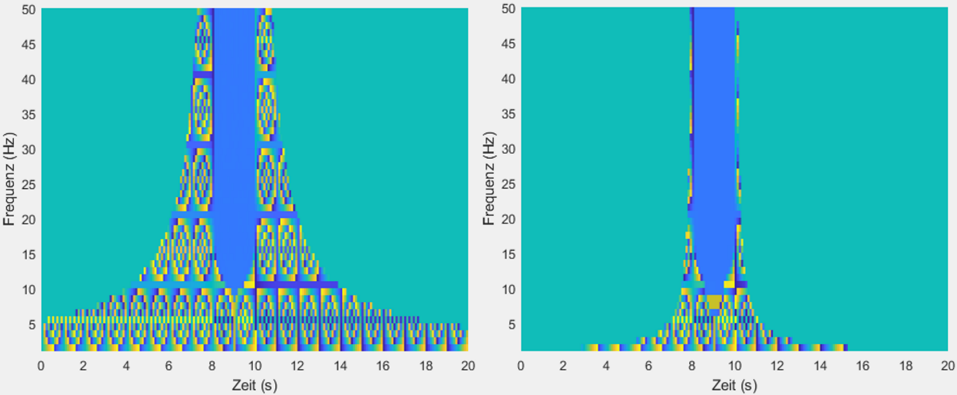
\includegraphics[width=0.5\textwidth]{papers/wavelets/images/13_CWT-CalcReduct.png}
	\caption{Reduktion der Berechnungen illustriert am Phasengang}
	\label{wavelet:fig:CwtCalcReduct}
\end{figure}

\subsection{Elimination der For - Schlaufen
	\label{wavelets:subsection:EliminationForSchlaufen}}
Die Rechenzeit konnte mit dem vorhergehenden Schritt nur minimal herabgesetzt werden. Ausserdem ist dieser Schritt auch nur dann zielführend, wenn im Messzeitraum nur wenig Signalanteile vorhanden sind (d.h. wie im Anwendungsfall nur kurzweilig etwas auftritt). Aus diesem Grund musste besserer Ansatz gewählt werden. 
Die neue Idee war, das Wavelet nicht ständig über die doppelten For-Schlaufe an den einzelnen Auswertungspunkten $x(n)$ errechnen zu müssen, sondern das Signal und das Wavelet als fertige Array mittels Skalarprodukt direkt zu verrechnen (Abbildung \ref{wavelet:fig:EliminationForLoops}).

\begin{figure}
	\centering
	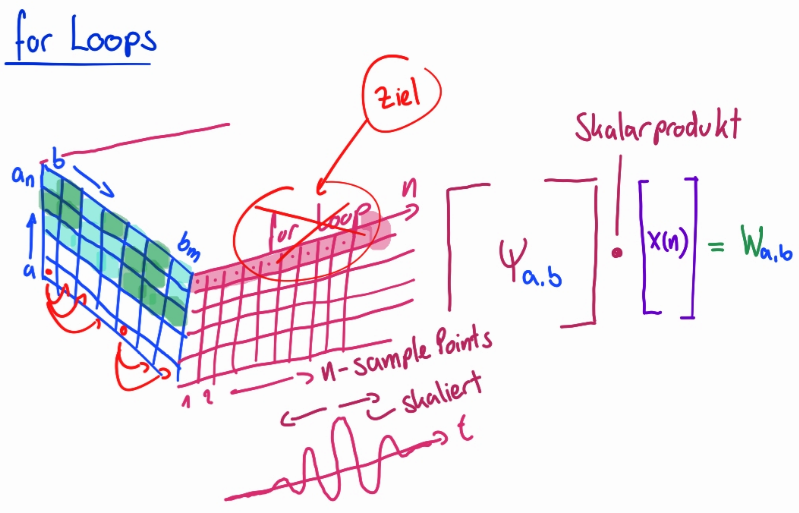
\includegraphics[width=0.5\textwidth]{papers/wavelets/images/14-1_EliminationForLoops.png}
	\caption{Zeitreduktion mittels direkter Skalarprodukt Verrechnung der Signal und Wavelet-Array}
	\label{wavelet:fig:EliminationForLoops}
\end{figure}

Die Abbildung \ref{wavelet:fig:EliminationForLoops} soll die Idee dahinter Erläutern. Die Frontfläche des Bildes (\ref{wavelet:fig:EliminationForLoops}) zeigt die beiden Laufvariablen $a$ (Frequenz) und $b$ (Verschiebung). Anstatt das für jede Position $a$, $b$ über eine weitere For-Schlaufe die einzelnen Werte zu erzeugen, wird wie in der Summenformel \[W_{a,b}=\sum_{a=f_0}^{a_n}\sum_{b=0}^{b_m}\frac{1}{N(a)}\sum_{n=0}^{N-1} x(n)\cdot\psi\left(\frac{t-b}{a}\right)\] neu direkt für jede Position $a$, $b$ ein Wavelet-Array erstellt. Ein solches Array kann in der Abbildung \ref{wavelet:fig:EliminationForLoops} als ein an der Stelle $a_n$ und $b_m$ in tiefenrichtung zeigendes Element des Quaders verstanden werden. Der Wert der Wavelettransformation wird danach direkt aus dem Skalarprodukt von einem solchen Arrayelement an der Stelle $a_n$, $b_m$ (also dem Wavelet mit der Frequenz $a_n$ und der zeitlichen Verschiebung $b_n$) sowie dem Signal $x(n)$ generiert.
Diese zeitliche Reduktion widerspiegelt sich auch im Code wieder (Abbildung \ref{wavelet:fig:EliminationForLoopCode}), weil dadurch zwei For-Schlaufen entfallen.

\begin{figure}
	\centering
	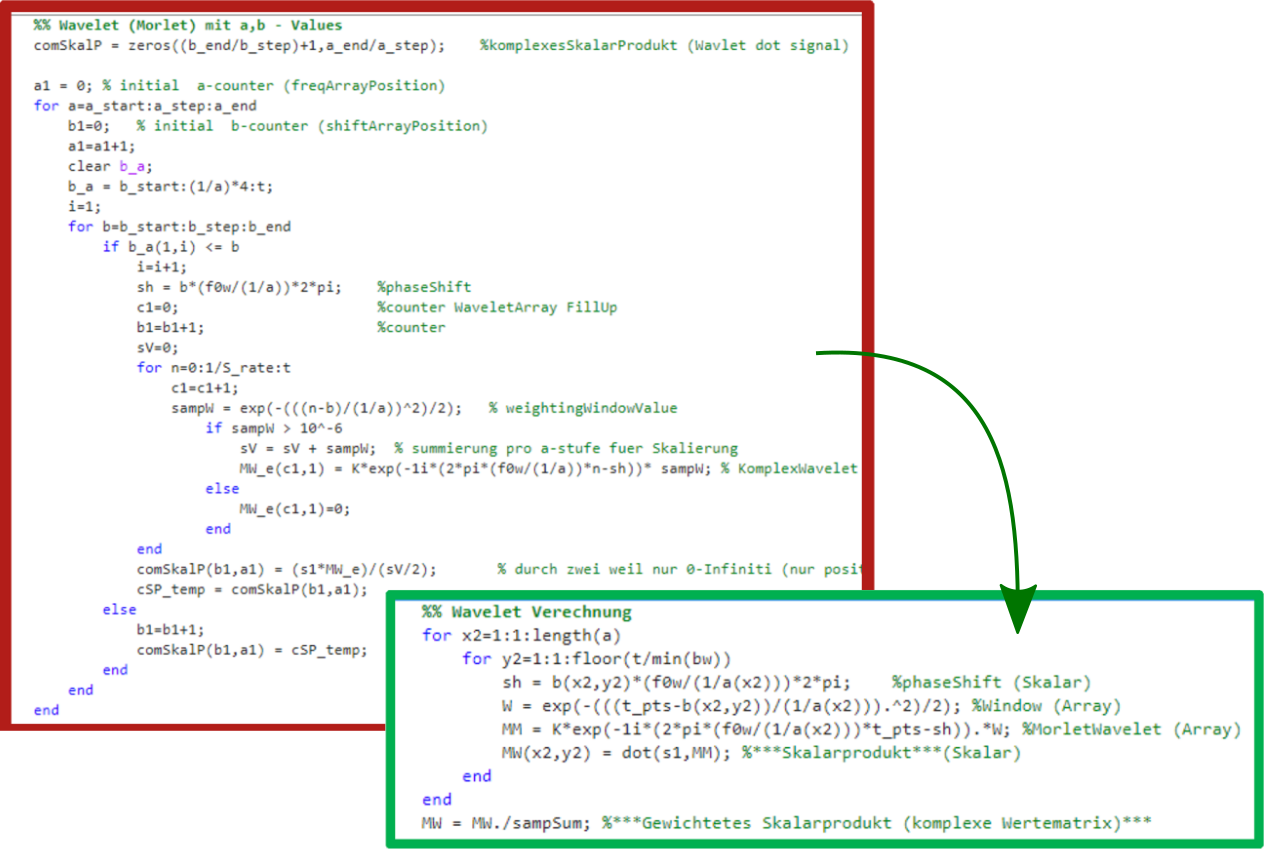
\includegraphics[width=\textwidth]{papers/wavelets/images/14-2_CodeSkalarProd.png}
	\caption{Code Reduktion durch Implementierung des Skalarproduktes zwischen Signal und Wavelet-Array. Diese visuelle Reduktion widerspiegelt sich auch in der Berechnungszeit des CWT-Programm.}
	\label{wavelet:fig:EliminationForLoopCode}
\end{figure}

\subsection{Adaptierter Zeitschritt
	\label{wavelets:subsection:AdaptierterZeitschritt}}
Der letzte Schritt um das Programm noch schneller zu machen, ist angelehnt an das Konzept der Filterbank bei der DWT (diskrete Wavelettransformation). Dabei soll die zeitliche Auflösung der Periodenbreite des Wavelets angepasst werden. Den ein tieffrequentes Wavelet besitzt eine zeitlich viel höhere Ausdehnung als ein hochfrequentes stark komprimiertes Wavelet (Abbildung \ref{wavelet:fig:adaptedShift_b}) und es ist nicht sinnvoll das Wavelet bei allen Frequenzen um dieselbe Zeitdauer zu verschieben.

\begin{figure}
	\centering
	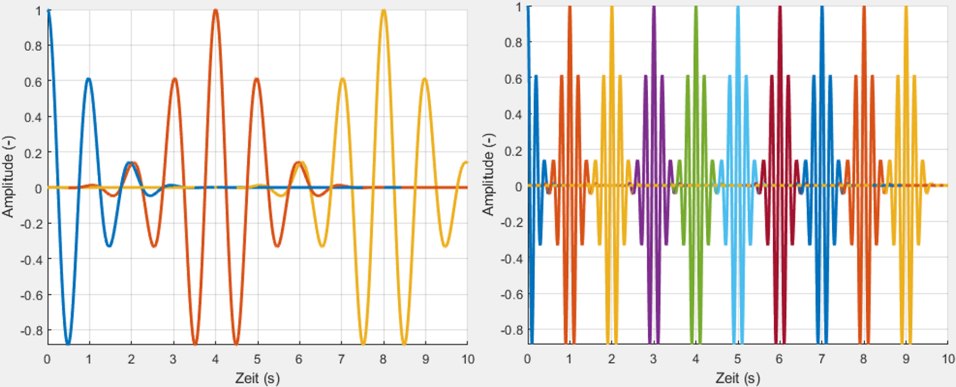
\includegraphics[width=0.5\textwidth]{papers/wavelets/images/15-1_adaptedShift-b.png}
	\caption{Darstellung der zeitlichen Ausdehnung eines Morlet Wavelets bei zwei unterschiedlichen Frequenzen.}
	\label{wavelet:fig:adaptedShift_b}
\end{figure}

Die Frequenzauflösung war schon einstellbar als Vielfaches der gewählten Grundfrequenz, was in dem Zusammenhang hier noch versucht wurde (spezifisch für das Filterbank adaptierte CWT), ist eine Frequenzerhöhung zu Radix zwei (d.h. $f_\text{wavelet} = 2^k$ pro Stufe $k = 0, 1, 2$ bis $K$). Dadurch kann eine Rasterung der $a$, $b$ Fläche wie im linken Bild \ref{wavelet:fig:adaptedFrequndTime} erzeugt werden.

\begin{figure}
	\centering
	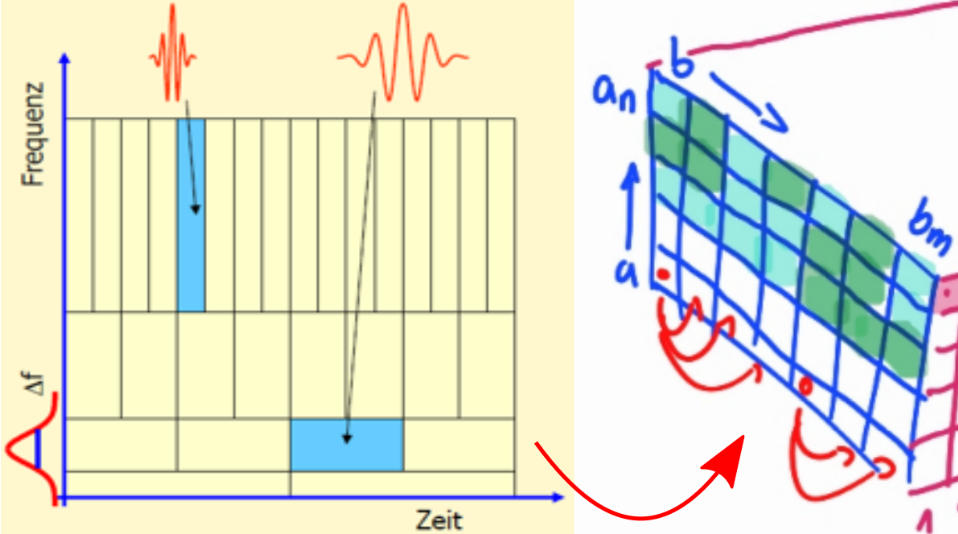
\includegraphics[width=0.35\textwidth]{papers/wavelets/images/15-2_adaptedFrequndTime.png}
	\caption{Variable Verschiebung sowie Skalierung angelehnt an die Idee der Filterbank bei der DWT. Im Programm umgesetzt an der $a_n$ x $b_m$ - Matrix}
	\label{wavelet:fig:adaptedFrequndTime}
\end{figure}

Dabei entsteht aber noch ein Problem, das es zu lösen gilt. Die Darstellung ist zwar eindeutig für das Verständnis, entspricht aber nicht einer $n$ x $m$ Matrix mit der man rechnen könnte.
Die Lösung dieses Problems ist andeutungsweise im rechten Bild mit den roten Pfeilen dargestellt. Die Anzahl an Spalten ist abhängig von der höchsten Frequenz und der dafür gewählten zeitlichen Verschiebung.
Für die zeitliche Verschiebung $b$, wurde ein $\Delta t=\frac{1}{a}\cdot4$ gewählt, da das gerade einer 50\% Überlappung entspricht. Die Anzahl Spalten ergibt sich demnach aus \[N_{spalten}=\frac{T_\text{signal}}{\frac{1}{a_{max}}}\cdot4.\] (Abbildung \ref{wavelet:fig:filterbankFillUp})

\begin{figure}
	\centering
	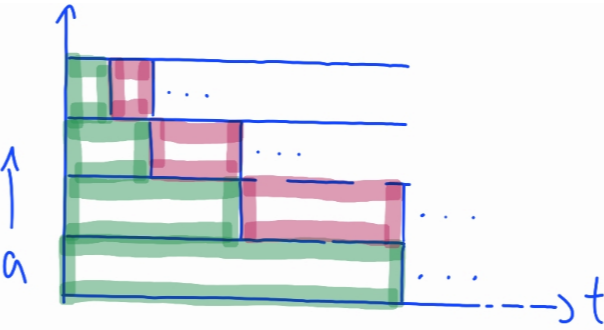
\includegraphics[width=0.3\textwidth]{papers/wavelets/images/16-1_filterbankFillUp_1.png}
	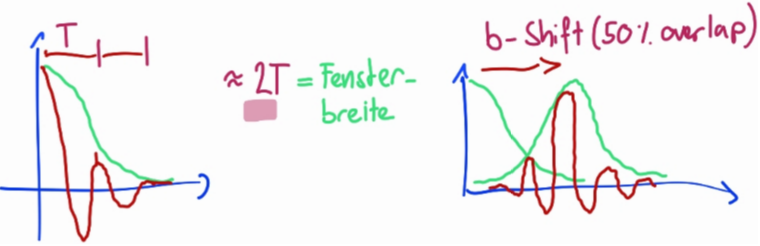
\includegraphics[width=0.4\textwidth]{papers/wavelets/images/16-2_filterbankFillUp_2.png}
	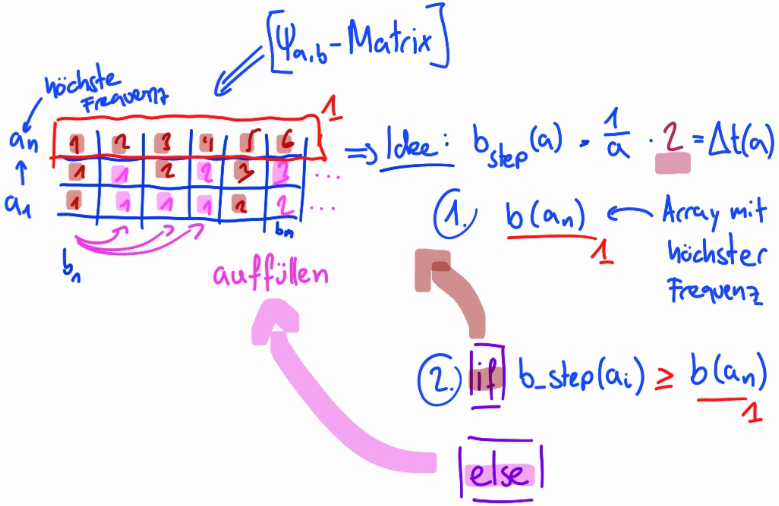
\includegraphics[width=0.4\textwidth]{papers/wavelets/images/16-3_filterbankFillUp_3.png}
	\caption{Schematische Idee hinter der Befüllung mit einem an die Frequenzskalierung $a$ angepassten Zeitschritt der Verschiebung $b$, inkl. pseudo-Code zur Matrixbefüllung.}
	\label{wavelet:fig:filterbankFillUp}
\end{figure}

Um diesen Befüllungsprozess zu veranschaulichen, im Folgenden ein kleines Beispiel für die Frequenzen 1Hz – $2^k$Hz, wobei $k_{max} = 3$. Die Skalierung $a$ wurde übrigens im Code so implementiert, dass sie direkt der Frequenz entspricht und nicht bloss eine Skalierung gegenüber der Grundfrequenz $f_0$ beschreibt. 

\begin{figure}
	\centering
	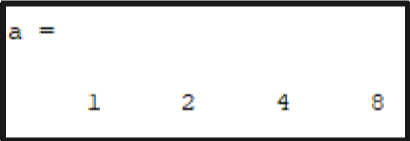
\includegraphics[width=0.2\textwidth]{papers/wavelets/images/17-1_a-Array.png}
	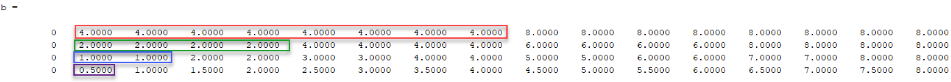
\includegraphics[width=\textwidth]{papers/wavelets/images/17-2_BspFillUp.png}
	\caption{Beispiel für die Matrixbefüllung wie sie im CWT-Code passiert (hier direkt angelehnt eine mit $2^k$ steigenden Frequenz $k$)}
	\label{wavelet:fig:BspFillUp}
\end{figure}

Für ein Signal mit einer Zeitdauer von 8s entstehen dadurch folgende Blöcke, für die zeitlichen Ausgaben pro Frequenz. Einfach ausgedrückt: 
überall da, wo die selbe Zahl steht pro Zeile, wird auch der selbe Wert ausgegeben. Es werden also nur noch Berechnungen an den Stellen gemacht wo es einen Wertewechsel pro Zeile gibt. Was genau der Abbildung \ref{wavelet:fig:BspFillUp} entspricht.

\subsection{Beispiel einer CWT mit Anlehnung an eine $2^k$ Filterbank analog zur DWT
	\label{wavelets:subsection:Radix2CWT}}
Die stetig halbierende Frequenzauflösung kann sowohl am Amplituden- als auch am Phasengang nachvollzogen werden. Natürlich ist quadratische Steigerung der Frequenz für eine CWT nicht wirklich sinnvoll, weil der Informationsverlust zwischen den betrachteten Frequenzen schnell sehr gross wird. Trotzdem brachte die Methode des Matrixbefüllen, also das einbringen eines frequenzangepassten Zeitschrittes, eine deutliche Steigerung der Rechenzeit bei kleinem Auflösungsverlust (Abbildung \ref{wavelet:fig:FilterbankAnwendung}).

\begin{figure}
	\centering
	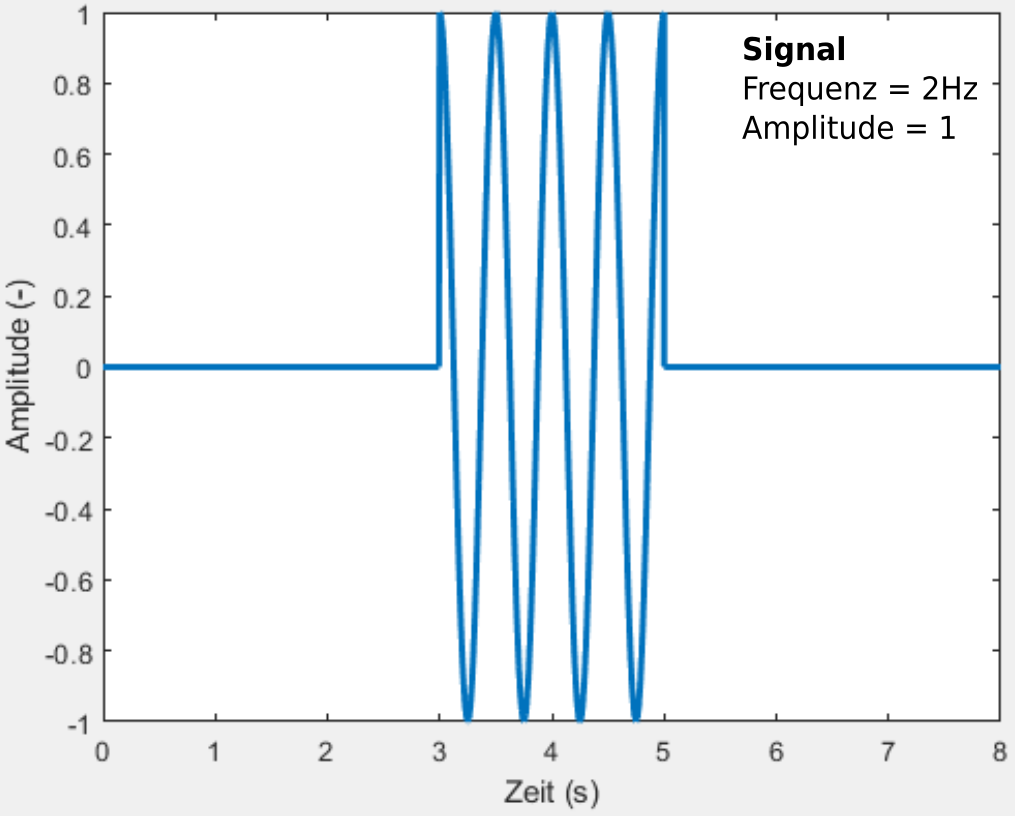
\includegraphics[width=0.2\textwidth]{papers/wavelets/images/17-3_AnwCwtFilterbankSig.png}
	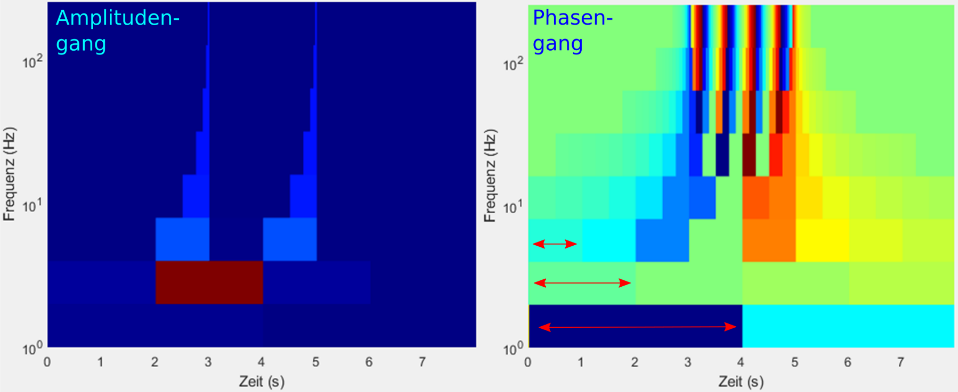
\includegraphics[width=0.75\textwidth]{papers/wavelets/images/17-3_CWT-FilterbankStyle.png}
	\caption{Bsp. 2Hz Signal untersucht mit einer CWT, mit Frequenzabstufung $2^k$, in Anlehnung an die DWT. Das halbieren der Auflösungsstufe ist an Amplituden- und Phasengang eindeutig zu erkennen}
	\label{wavelet:fig:FilterbankAnwendung}
\end{figure}

